\section{Para-real method}
	
Para-real method is a parallel-in-time integration methods which was introduced in 2001 by Lions, Maday and Turinici. Parareal computes the numerical solution for multiple time steps in parallel, it is categorized as a parallel across the steps method.

\subsection{Explanation}

As for the previous methods, we consider an initial value problem of the form :

$$\left\{\begin{aligned}
    X'&=f(t,X) \qquad t_0\le t\le T \\
    X(t_0)&=X_0
\end{aligned}\right.$$

\noindent Parareal method need a decomposition of the time interval $[t_0,T]$ into $P$ slices $[t_j,t_{j+1}]$ with  $j\in\{0,\dots,P-1\}$ where $P$ is the number of process units. We also try to parallelize the algorithm so each time slice is assigned to one process. We denote by $F$ a function which is of high accuracy and and $G$ which is of low accuracy. That is to say that $F$ will be very expensive in terms of calculation but very accurate and $G$ will be very cheap.  \\

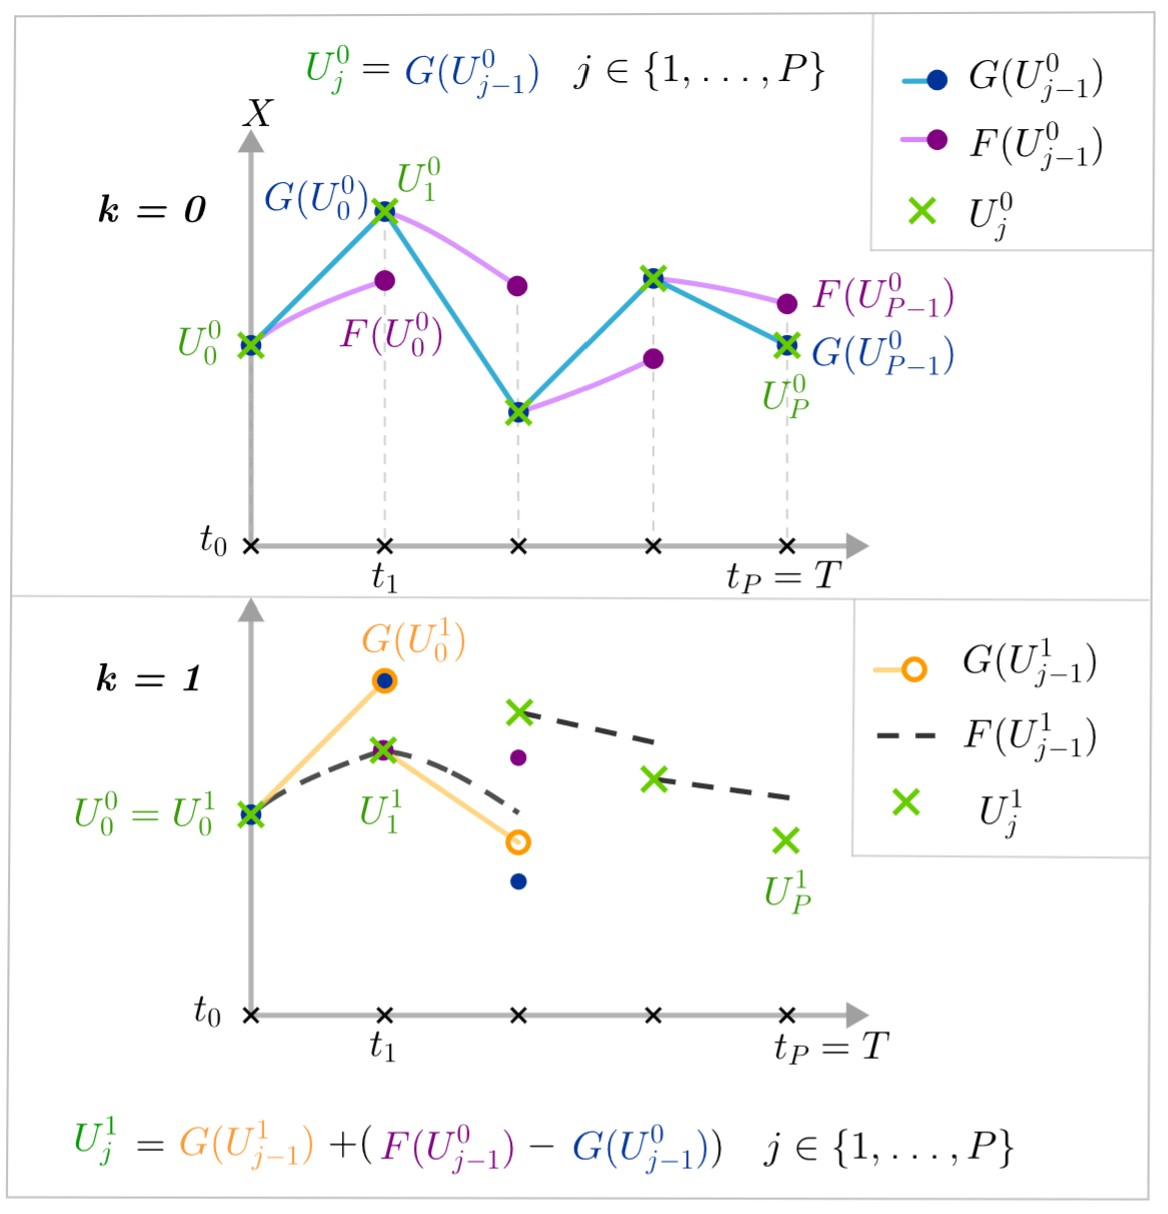
\includegraphics[width=\textwidth]{"images/schema_parareal.jpg"}

\subsection{Application to the Lorenz system}

We try now to apply this method on the Lorenz system. In the previous explanation, we have also :

$$X'=\begin{pmatrix}
    x' \\
    y' \\
    z'
\end{pmatrix}, \quad X=\begin{pmatrix}
    x \\
    y \\
    z
\end{pmatrix} \quad et \quad f(t,X)=\begin{pmatrix}
    \sigma(y-x) \\
    x(r-z)-y \\
    xy-bz
\end{pmatrix}$$

\noindent For the two integrators we will take Runge Kutta order 4 method which a litle time step for $F$ and a larger one for $G$.
